\scanpage{156}
\mspage{79}
% archive sheet number: 155
% L1–3
Soit
\[
\begin{aligned}
 T=T_{D_0}&=\text{stabilisateur de }D_0\text{ dans }G_{s_0}\\
 &=\{g\in G_{s_0}\mid\underset{\text{i.e. }g(t_0)\in D_0}{g(D_0)=D_0}\}
\end{aligned}\tag*{(75)}
\]
% L4–6
\deleted{Posons} On a donc
\diagram{\[
\begin{tikzcd}[ampersand replacement=\&,row sep=0.5em,column sep=0.4em]
G^+_{0s_0}=\deleted{\unsure{T|\mathcal U}}U_{\deleted{\unsure{s_0}}}\subset \& G_{s_0} \& =\overset{\deleted{\unsure{B}}}{B'}\\
\& T_{\deleted{\unsure{0}}}\arrow[u,phantom,"\rotatebox{90}{$\subset$}" description] \& ,
\end{tikzcd}
\]}
% L7–8
\deleted{quel est $T\cap G_0^+$} je dis que
\[
T\cap G_0^+=\{1\},\qquad T\xrightarrow{\chi\mid T}(\mathbb Z/n\mathbb Z)^*
\quad\text{épi donc iso}\ \deleted{\unsure{,}}
\tag*{(76)}
\]
% L9–11
en d'autres termes, je dis que $T$ définit un \uline{scindage} de la structure d'ext. (71)
\[
G_{s_0}\simeq\deleted{\unsure{G_{s_0}}}
\underbrace{U}_{G^+_{0s_0}\simeq\underbrace{\mathbb Z/n\mathbb Z}_{\text{non can.}\unsure{^{\mathrm t}|!}}}.
\underset{\substack{\wr\Vert\\(\mathbb Z/n\mathbb Z)^*}}{T}\quad 1/2\ \text{direct}\ .
\tag*{(77)}
\]
% L12–14
Soit donc $g\in G^+_{0s_0}$ qui soit dans $T$ i.e. tel que $g(t_0)\in D_0$ donc $g(t_0)=\dot\lambda t_0$ ($\dot\lambda\in Z$), \deleted{comme $g\in G_0$ et $g$ fixe $s_0$, \unsure{on voit} il s'ensuit que $\{s_0,t_0\}$ et $\{gs_0=s_0,g(t_0)\}$ appartiennent à la $=$ structure $P_{i_0}$ ($i_0\in\Pi$), mais $g(t_0)=\dot\lambda t_0$ \deleted{signifie}\inserted{implique} que} Soit
% L17
\[
i_0=\tau_A(\{s_0,t_0\}),\quad i_1=\tau_A(\{\underset{\substack{\Vert\\g(s_0)}}{s_0},g(t_0)\})
\]
% L18–21
comme on a $g\in G_0$ et $g(s_0)=s_0$, on a donc
\[
i_1=g(i_0)=i_0
\]
et comme $g(t_0)=\lambda.t_0$, on a
\[
i_1=T_\lambda.i_0\qquad\text{d'où}\quad \lambda=1,\quad\text{i.e. }g(t_0)=t_0
\]
% L22–24
\deleted{[on aurait pu dégager : deux points différents d'un rayon, \deleted{\unsure{reliés}} \inserted{$A$-adjacents} à un même $s$, donnent}
\figure{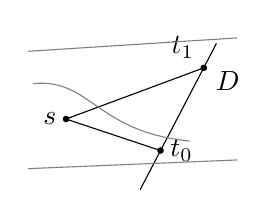
\begin{tikzpicture}[x=1cm,y=1cm,baseline]
\coordinate (s) at (0,0);\coordinate (tzero) at (1.2,-.4);\coordinate (tone) at (1.75,.65);
\draw (s)--(tone) (s)--(tzero) (.94,-.9)--(1.91,.96);
\fill (s) circle (1.2pt) node[left] {$s$};
\fill (tone) circle (1.2pt) node[above left] {$t_1$};
\fill (tzero) circle (1.2pt) node[right] {$t_0$};
\node[right] at (1.78,.48) {$D$};
\draw[gray] (-.48,.86)--(2.17,1.03) (-.48,-.63)--(2.17,-.52);
\draw[gray] (-.42,.45) .. controls (.32,.52) and (.37,-.16) .. (1.57,-.28);
\end{tikzpicture}}
